% !TeX spellcheck = en_US

\chapter{Plastic Mulching in Agriculture}
\label{ch:plastic-mulching}

\paragraph{Abstract} Plastic mulching\marginnote{This chapter is based on: \fullcite{SteinmetzPlastic2016}.\par See \nameref{ch:author-contributions}, page~\pageref{ch:author-contributions}, for details.} has become a globally applied agricultural practice for its instant economic benefits such as higher yields, earlier harvests, improved fruit quality, and increased water use efficiency. However, knowledge of the sustainability of plastic mulching remains vague in terms of both an environmental and agronomic perspective. This chapter critically discusses the current understanding of the environmental impact of plastic mulch use by linking knowledge of agricultural benefits and research on the life cycle of plastic mulches with direct and indirect implications for long\-/term soil quality and ecosystem services. Adverse effects may arise from plastic additives, enhanced pesticide runoff, and plastic residues likely to fragment into micro- or nanoplastics but remaining chemically intact and accumulating in soil where they can successively sorb agrochemicals. The quantification of plastic debris in soil remains challenging due to the lack of appropriate analytical techniques. The cost and effort of recovering and recycling used mulching films may offset the aforementioned benefits in the long term. However, comparative and long\-/term agronomic assessments have not yet been conducted. Furthermore, plastic mulches have the potential to alter the soil quality by shifting the edaphic biocoenosis, accelerate \ch{C/N} metabolism eventually depleting \ac{som} stocks, increase soil water repellency, and favor the release of greenhouse gases. A substantial process understanding of the interactions between the soil microclimate, water supply, and biological activity under plastic mulches is still lacking but required to estimate potential risks for long\-/term soil quality. Currently, farmers mostly base their decision to apply plastic mulches rather on expected short\-/term benefits than on the consideration of long\-/term consequences. Future interdisciplinary research should therefore gain a deeper understanding of the incentives for farmers and public perception from both a psychological and economic perspective to develop new support strategies for the transition into a more environment\-/friendly food production.

\section{Introduction}
\label{sec:plastic-mulching:intro}

Rapid population growth poses a major challenge for both efficient and sustainable agricultural practices given the limited availability of arable land. In order to meet the increasing food demand \citep{GodfrayFood2010}, plastic mulching has become a widely used technique for its instant economic benefits such as higher yields and improved crop quality \citep{LamontPlastic1993}. However, after six decades of research\sidenote{See \citet{KasirajanPolyethylene2012} for an extensive historical review.}, the knowledge of the sustainability of plastic mulches remains vague in terms of both an environmental and agronomic perspective.

Plastic mulches are primarily used to protect seedlings and shoots through insulation and evaporation prevention, thus maintaining or slightly increasing soil temperature and humidity \citep{TararaMicroclimate2000}. Furthermore, the application of plastic covers is known to reduce weed and pest pressure \citep{McKenzieLandscape2001}. Often reported benefits are minimization of the development time for seed and fruit, yield increase, the prevention of soil erosion and weed growth, and consequently reduction of herbicide and fertilizer use \citep{Chalker-ScottImpact2007,EspiPlastic2006,LamontPlastic1993, Scarascia-MugnozzaPlastic2011}. These prospects have made plastic films an upcoming technology, nowadays making up by far the largest proportion of covered agricultural surface
in Europe (\SI{4270}{\square\kilo\meter}), an area four times larger than that covered by greenhouses and six times that of low tunnels \citep{Scarascia-MugnozzaPlastic2011}. While the agricultural surface covered with mulching films remains constant or shows only slightly growing trends throughout the world (\SI{5.7}{\percent} annual growth until 2019) \citep{TransparencyMarketResearchAgricultural2013}, the covering rate in China increased dramatically between 1991 and 2004 with a growth rate of \SI{30}{\percent} per year \citep{EspiPlastic2006}. The \citet{NationalBureauofStatisticsofChinaChina2012} reported a four-fold increase of plastic mulch use from \SIrange[range-phrase = { to }]{319}{1245}{\mega\tonne} between 1991 and 2011.

However, the modification of the microclimatic conditions under plastic mulches not only enhances plant productivity but also increases biological degradation of litter and \ac{som}, which has recently been discussed as a trigger to rapid depletion of soil nutrients in general and carbon stocks in particular \citep{Domagala-SwiatkiewiczEffect2013,ZhangEffects2015}. This may eventually reduce soil quality in terms of impeding the soil's capability to serve its intended purpose \citep{DoranDefining1994}.
Furthermore, the excessive use of hardly degradable \ac{pe} has been apprehended to lead to substantial amounts of plastic waste residues accumulating each year \citep{AlbertssonMechanism1987}. This, in turn, may potentially release toxic additives into the soil \citep{RamosPolyethylene2015}.

The majority of reviews published on agricultural plastic mulching strongly focuses on the feasibility or efficacy assessments of biodegradable films \citep{BrodhagenBiodegradable2015,KasirajanPolyethylene2012} which have so far been hardly accepted as a functional alternative to \ac{pe}. More general contributions compared various synthetic and natural mulching materials with each other \citep{Chalker-ScottImpact2007,GreerAluminum2003} or with respect to certain agricultural practices, such as ridge\-/furrow systems \citep{GanRidgeFurrow2013} and integrated weed control \citep{BondNonchemical2001,CaseReview2005}. The first and most general reviews published on plastic mulching \citep{LamontPlastic1993,TararaMicroclimate2000} were animated with the beneficial prospects of plastic mulch use, however, merely discussing potential drawbacks. This trend still applies to the majority of current research articles emphasizing individual effects of plastic mulching with particular focus on short\-/term agronomic benefits \citep[for instance,][]{HeRice2013,Lopez-LopezWater2015,WangCombination2010}. In contrast, the long\-/term impact of plastic mulching as a standard agricultural practice is still virtually unknown in terms of potentially deteriorating soil quality or their post\-/crop fate, and therefore presents a challenge to bear a holistic sustainability evaluation. For this, it is important to combine the various results from individual studies to derive a system\-/based and interdisciplinary understanding of the processes governing the impact of plastic mulches on agroecosystems.

This review aims at evaluating the sustainability of plastic mulch use in agriculture from the perspective of soil biogeochemistry, environmental chemistry, agronomy, and society. We link current knowledge of agricultural benefits and research on the fate and life cycle of plastic mulches with direct and indirect implications of plastic mulching for short- and long\-/term soil quality. In this respect, we first outline the fate of \ac{pe} mulches while in use and after their life cycle has come to an end by explaining possible degradation pathways of buried mulch fragments. In addition to the fate of the plastic itself, we evaluate the long\-/term impact of plastic mulches on soil quality with respect to microbial diversity and \ac{som} composition and degradation, both important but often neglected factors influencing ecosystem functions \citep{PowerEcosystem2010}. On this basis, we assess the value of plastic mulches in an agronomic context in order to provide first insights into its sustainability. We finally identify the need of research for a better comprehension of the processes and factors influencing wanted and unwanted effects of agricultural plastic mulches.

\section{Methods}
\label{sec:plastic-mulching:methods}

We searched both Web of Science and Google Scholar literature data bases for search terms including plastic or \ac{pe} mulch, cover, film, or tarp used in agriculture\sidenote{\sloppy Exact search string: \texttt{(plastic* OR \acl{pe}) AND (mulch* OR cover* OR film OR tarp) AND (soil OR agricultur*)}.}. Based on these findings and supplemented with cross references, we selected \num{572}~original research articles, \num{53}~reviews, \num{23}~books or book chapters, \num{21}~reports and doctoral theses, and \num{7}~patents and industrial standards for further evaluation. The literature covered the following major subtopics: use, properties, fate, impact on soil quality, and economic effects. For a more comprehensive perspective on the economics of plastic mulches we selected and followed the concept of ecosystem services \citep{MillenniumEcosystemAssessmentEcosystems2005} to identify economic elements linked to plastic mulching and to provide an integral overview of the current state of agronomic knowledge of the impacts of plastic mulch.

\section{Use and Properties of Plastic Mulches}
\label{sec:plastic-mulching:use-and-properties}

The largest benefits plastic mulches are used for on immense scales worldwide stem from their distinct optical and material properties that allow transmission or reflectance of specific wavelengths of incoming solar radiation \citep{BrownBlack2001,Chalker-ScottImpact2007,CsizinszkyColor1995,GordonPlastic2008,HaynesUse1987}. In order to produce highly customizable materials with high flexibility, durability, easy processing, and freedom from odor and toxicity \citep{WrightIns2019}, \ac{pe} has become by far the most frequently used base material in agricultural mulch production \citep{Diaz-PerezBell2010,KaraEffects2013,LocascioRed2005,SivanNew2011}. Its properties are usually modified by additives such as plasticizers, colored pigments, \ac{uv} stabilizers, or other polymers. The main types of \ac{pe} used in agriculture are low- and high-density \ac{pe} and linear low-density \ac{pe}.
High-density \ac{pe} is used to reduce weight and cost, contributes to the tear strength of the material, and provides a reliable moisture barrier \citep{LamontPlastics2005}. Linear low-density \ac{pe} is used for its elasticity and high puncture resistance \citep{AnthonyMultilayer1983}. Numerous other \ac{pe} mulching variations have already been patented, for instance composite mulches such as paper covered in styrene butadiene latex \citep{DalebrouxMulching1997}.
\citet{SabbaghAgricultural2010} patented a non\-/degradable and mechanically stable mulch barrier consisting of low-density \ac{pe}, linear low-density \ac{pe}, and \ac{pa}\slash nylon impermeable to soil fumigants. However, the degradability of such materials, the tendency to create microplastic debris, and their practical application are unknown. Mulches containing \ac{pvc} were prohibited for mulching in the US for their toxicity and carcinogenic potential \citep{USEPAGuidelines2012} and have been restricted to greenhouse covering and irrigation pipes \citep{Scarascia-MugnozzaPlastic2011}. In order to achieve longer life cycles of three years or more \citep{BrucknerSpargelanbau2008} as specifically needed for strawberries and asparagus growth, \ac{eva} and \ac{eba} are added to \ac{pe} mulches as co-polymers \citep{EspiPlastic2006}.

Although this depends on regional climatic conditions and land use practices, maximum yields are mainly achieved by optimizing the amount of solar radiation absorbed by the crop. Further microclimatic parameters to be modified include the root zone and leaf temperature, humidity, and therewith soil moisture and plant transpiration rates, for example to manage soil temperatures at night or in colder regions by preventing evaporative cooling and emission of long\-/wave radiation from the soil \citep{HamOptical1993}. This is achieved by controlling the gas and heat exchange between the soil and the environment \citep{LamontPlastic1993,TararaMicroclimate2000}. For such purposes, black, transparent, and white mulches are the colors used most commonly. However, the color selection strongly depends on the crop type and the crop's environment, as well as the temperature that can be tolerated by plants and seedlings \citep{LamontPlastic1993,TararaMicroclimate2000}.

Black is the predominant mulch color since it can both absorb and re-emit radiation as thermal energy or long\-/wavelength \ac{ir} \citep{LamontPlastic1993,LamontPlastics2005}. Black mulch\-es are favored in moderate climate zones in order to increase soil warming by up to \SI{6}{\degreeCelsius} and double soil moisture, resulting in extended growing seasons. In very hot regions or for special use cases such as asparagus growing, white or white\-/on\-/black mulches are used to maintain or slightly lower soil temperatures by up to \SI{2}{\degreeCelsius} compared to bare soil \citep{HamOptical1993,HeissnerComparison2005}. The effects of plastic mulches on soil temperature and moisture typically decrease with soil depth, becoming mostly insignificant below \SI{40}{\centi\meter} \citep{Diaz-HernandezEffects2012,HeissnerComparison2005}. By contrast, transparent plastic films are poor absorbers of solar radiation but able to transmit \SIrange{85}{95}{\percent} of radiation \citep{HamOptical1993}. The condensed water below the film surface absorbs the \ac{ir} radiation reflected by the soil so that the heat is retained. This greenhouse effect makes transparent films profitable in colder regions \citep[for instance,][]{HaynesUse1987,StreckEffect1995}. However, the disadvantage of the high transmittance properties of transparent mulches is the lack of weed control, which continue to grow when exposed to sun light \citep{LamontPlastic1993}. In arid regions, transparent films are primarily used for soil solarization due to the extraordinarily high temperatures occurring under transparent mulches. Soil solarization is a soil sterilization method applied before planting to eradicate soilborne pathogens and devitalize weed growth \citep{HorowitzSolarization1983,TamiettiSoil2006}. In addition, photoselective films are capable of reflecting \ac{par} to above\-/film leaves and transmitting \ac{ir} light, representing a compromise between transparent and black mulches \citep{PaulUse2005}. For pest and pathogen control, pesticide \citep{SubrahmaniyanWeed2011} or aluminum \citep{CsizinszkyColor1995} coatings may additionally be applied\sidenote{See \citet{GreerAluminum2003} for a detailed overview.}. Other colors such as red, blue, yellow, or orange have also been tested for special requirements in vegetable production such as repelling certain pests or attracting beneficial insects \citep{CsizinszkyColor1995,LamontPainting1990, OrzolekUse1993}.

Apart from the evaluation of specifically intended effects of the variety of different plastic materials, none of the aforementioned studies focused on implications for other soil processes. In order to assess the impact of plastic mulching on soil quality, the current focus on the evaluation and optimization of the benefits of plastic mulching must be extended by the evaluation of potential unwanted side effects in soil and surrounding ecosystems. A comprehensive understanding of these effects will require an integrated assessment of application\-/specific impacts as well as process\-/orientated research on soil quality and the fate of mulch residues in soil that both the mulch and the soil are subjected to with respect to different environmental and agricultural conditions in particular regions of the world. In the following sections, we will thus discuss the current knowledge of these aspects.

\section{Fate of Plastic Mulches and their Additives}
\label{sec:plastic-mulching:fate}

\subsection{Life Cycle and Degradability of \Acs{pe}}
\label{sec:plastic-mulching:life-cycle}

A polymer is typically defined as ``environmentally degradable'' or ``biologically degradable'' if it has the ability to undergo disintegration, this is deterioration in mechanical properties, possible fragmentation, followed by microbial attack \citep{KrzanStandardization2006}. European standards further define that after six months more than \SI{90}{\percent} of the initial compound must be broken down to biomass, water, and \ch{CO2} \citep{DINEN13432Packaging2000}. In this sense, chemically inert \ac{pe} can be treated as virtually non\-/biodegradable \citep{AlbertssonMechanism1987}. Studies on the degradability of \ac{pe} have been recently reviewed in two articles \citep{KruegerProspects2015,Restrepo-FlorezMicrobial2014}. They reported that \ac{pe} degradation takes place to a certain extent. However, the authors agreed that this process is very slow under environmental conditions. Although the stability of \ac{pe} is beneficial for the lifetime extension of the mulch in use, this inertness is likewise the most problematic property concerning the disposal of used mulch films.

The typical application time of plastic mulches in agriculture lasts only a few months and can be reduced even further when exposed to extreme weather events such as hail and storms due to physical fragmentation and chemical aging processes \citep{Scarascia-MugnozzaPlastic2011}. More resilient mulches are required for perennial crops like strawberry or asparagus \citep{HablotEffect2014}. The thinner the film the more difficult and time consuming it becomes to remove the complete film from the field at the end of a crop cycle without leaving residues in the soil. For this reason, plastic films or parts thereof are often intentionally or unintentionally left on the field to be further broken down mechanically \citep{MorenoImage2014}.
Despite its high relevance, there is no information up to now on the amount of plastic residues in soil. However, \num{10}-year laboratory experiments showed that low-density \ac{pe} buried in soil reduced its weight by only \SI{0.2}{\percent} per year \citep{AlbertssonMechanism1987}. Long\-/term (\numrange{32}{37}~years) studies by \citet{OhtakeStudies1998} estimated a period of approximately \num{300}~years required for complete degradation of a \SI{60}{\micro\meter} thin low-density \ac{pe} layer. In pure \ac{pe} without any degradation\-/promoting additives, polymer chain scission is, if at all, a very slow process. \ac{pe} mulches are resistant to hydrolysis and are not readily attacked by microorganisms \citep{StevensGreen2002}. The most efficient way of chemical degradation involves a photo\-/oxidation step when exposed to sunlight. During this process, carbonyl groups are formed which can be attacked by microorganisms so that the polymeric chains are broken down further. These processes are summarized as oxodegradation, this is the fragmentation of plastic under the influence of \ac{uv} radiation and temperature \citep{SivanNew2011}. According to the definition of the American Society for Testing and Materials \citep{ASTMD5488-94Terminology1994}, such processes cannot be referred to as biodegradation since carbonyl formation during photo\-/oxidation is not an enzymatic activity. Moreover, mulching films that are buried in the soil are not subject to photo\-/oxidation and therefore unlikely to be attacked by microorganisms due to the lack of carbonyl formation \citep{MorenoImage2014}.

If not removed from the field, plastic waste accumulates in the environment where it may pose a considerable threat to terrestrial and aquatic wildlife when taken up in the food chain \citep{BarnesAccumulation2009,DuisMicroplastics2016,RilligMicroplastic2012,SivanNew2011,TeutenTransport2009}. Eventually, the plastic loses its integrity and breaks down into smaller and smaller particles for which the term ``microplastics'' was coined by \citet{ThompsonLost2004}. Although numerous articles have already reported the formation of plastic residues of various sizes (\SI{700}{\square\micro\meter} to \SI{2850}{\square\centi\meter}) originating from mulching \citep[for example,][]{BriassoulisAnalysis2015,FeuilloleyDegradation2005,KyrikouBiodegradation2007,RamosPolyethylene2015}, the assessment of their fate in soil is still challenged for the development of adequate analytical methods to detect and quantify plastic residues in complex, heterogeneous environmental matrices \citep{RilligMicroplastic2012}. Recently, \citet{DumichenAnalysis2015} suggested a first approach for the determination of \ac{pe} plastic debris in solid media using \ac{ted-gc-ms}. However, the authors stressed the need for further research in terms of improving \ac{ted-gc-ms} measurements as well as developing alternative techniques for the quantification of other polymer types in different environmental media.

The compiled findings suggest a successive enrichment of the plastic residues in the soil---whether or not they are left in the soil intentionally or unintentionally. For a more detailed assessment of the environmental fate of plastic residues, a more comprehensive understanding of the fate of plastic debris in soil is essential. This assessment, however, urgently requires further advances in analytical techniques to detect, identify, and quantify plastic debris in heterogeneous samples like soil.

\subsection{Phthalates}
\label{sec:plastic-mulching:phthalates}

Among typical \ac{pe} mulch additives, plasticizing agents from the group of \acp{pae} with its model compound \ac{dehp} belong to the most discussed soil contaminants \citep{FuUptake2011,MagdouliDi2013,WangSoil2013}. Similar to other \acp{pae}, \ac{dehp} is suspected of being carcinogenic and endocrine\-/disrupting \citep{ErkekogluGenotoxicity2014}. The fate of such compounds is highly relevant when assessing the risks potentially originating from plastic mulches. However, demonstrating a connection between plastic mulch application and elevated \ac{pae} concentrations in soil or plants is not trivial since agrochemicals, wastewater irrigation, and atmospheric background concentrations represent further potential \ac{pae} sources \citep{HongjunDistribution2013,WangSoil2013,HeContamination2014}. In \ac{pe} mulches, \ac{pae} are only loosely incorporated in the polymer structure without covalent bonding and can therefore be leached out easily. Even \ac{pae} derivatives with low water solubility, low vapor pressure, and high \acp{kow} such as \ac{dehp} \citep{MagdouliDi2013}, have been found ubiquitously in the environment \citep{FernandezOccurrence2012}. While typical background concentrations of \acp{pae} in soil vary between \SIrange[range-phrase = { and }]{0.2}{33.6}{\milli\gram\per\kilo\gram} \citep{ZengPhthalate2008}, \ac{pae} levels in plastic mulches were detected in ranges from \SIrange[range-phrase = { to }]{50}{120}{\milli\gram\per\kilo\gram} \citep{WangSoil2013}.
Plastic\-/mulched crop land revealed concentrations of six major \acp{pae} between \SIrange[range-phrase = { and }]{74}{208}{\percent} higher than in non\-/mulched farmlands in China \citep{KongDiversities2012}. Most concentrations of \ac{dehp} and \ac{dbp} found in Chinese\-/grown vegetables and soil exceeded US and EU food security standards and environmental risk limits of \SIlist{0.7;1.0}{\milli\gram\per\kilo\gram}, respectively \citep{vanWezelEnvironmental2000,WangOccurrence2015}.

Once released from the mulching film, \ac{pae} may be distributed in environmental compartments by plant uptake, evaporation into the atmosphere, and runoff into groundwater and surface waters \citep{HeContamination2014}. In soil, \ac{pae} are degraded by microorganisms to different extent in dependence of the ester chain length. While short\-/chain esters, such as \ac{dep}, are to a certain extent susceptible to biodegradation, longer chains as in \ac{dehp} render the \ac{pae} persistent. When subjected to \ac{uv} radiation, \acp{pae} can degrade to phthalate monoesters and phthalic acid \citep{HankettMolecular2013}. In natural environments, the governing microbial degradation processes are hydrolysis, both aerobic and anaerobic, followed by aromatic ring cleavage \citep{MagdouliDi2013,StaplesEnvironmental1997}. Furthermore, microbial degradation of \acp{pae} is dependent on its metabolic yield: Whereas \ac{dep} is rapidly degraded and assimilated, \ac{dehp} and bis(2-ethylhexyl) adipate are more recalcitrant and only cometabolically degraded in the presence of an additional carbon source \citep{CartwrightDegradation2000,NalliBiodegradation2002}. This typically results in the formation of ethylhexanoic acid and ethylhexanol, both toxic to aquatic organisms and particularly resistant to further degradation \citep{HornPlasticizer2004}. Although laboratory\-/derived half lives of \acp{pae} in soil range from days to months, current research rather suggests that at least some of them persist for significantly longer periods in soil \citep{RudelDegradation1993}. Thus, the use of plasticizer\-/containing mulches involves a clear potential for accumulation of these xenobiotics in soil and a successively increasing risk of bioaccumulation and biomagnification in the food web.

Besides affecting the abundance and diversity of soil organism communities, crop quality can be impaired significantly when \acp{pae} are taken up by plants \citep{KapanenPerformance2008,WangOccurrence2015}. Through this pathway, phthalates may eventually enter the food supply chain representing an additional and probably significant source of exposure to humans.

\subsection{Polymer Degradation-Promoting Agents}
\label{sec:plastic-mulching:oxodegradation}

Due to the generally known high persistence of plastic residues and their additives in soil, the development of biodegradable plastics or the promotion of biodegradation of plastic materials is a promising option to avoid the accumulation of plastic in soil. First attempts were made to use different bacterial strains, for example from the gut of the Indian meal moth (\latin{Plodia interpunctella}), which were able to degrade \SIrange{6}{10}{\percent} \ac{pe} during a \SI{60}{\day} incubation period \citep{HadadBiodegradation2005,KruegerProspects2015,YangPlastic2015}. However, such selective treatments have been restricted to laboratory conditions. They seem both too difficult and expensive to be applied on large agricultural scales and bear the risk of potentially introducing invasive or detrimental species into productive systems. Certain agrochemicals, such as paraquat and mancozeb were found to accelerate the oxidation rate and embrittlement of the \ac{pe} foil during laboratory experiments, while sulfur and chlorpyrifos did not show significant effects \citep{YehEffect2015}. By contrast, various types of other \ac{pe} additives have already been successfully tested and applied for their ability to promote the breakdown of mulches. \Citet{KyrikouBiodegradation2007} provided a comprehensive collection of data on various types of mulches and investigated under which conditions and to which extent they are (bio)degradable. In order to promote oxodegradation, additives can be used to facilitate chain cleavage and microbial attack. Polymer breakdown is induced by radicals produced by pro\-/oxidants and the subsequent production of oxidized carbon chains \citep{BriassoulisDegradation2015}.
Such pro\-/oxidants mainly contain carbonyl groups and compounds containing transition metals like \ch{Fe}, \ch{Co}, and \ch{Mn} \citep{KyrikouBiodegradation2007}. However, added organic compounds or metals of environmental concern may lead to increasing soil contamination \citep{KoutnyBiodegradation2006,Scarascia-MugnozzaPlastic2011}. It has not yet been satisfactorily shown to what extent the oxidation products are truly biodegradable under realistic environmental conditions. In several standardized laboratory biodegradability tests, less than \SI{2}{\percent} of a pro\-/oxidant\-/containing \ac{pe} mulch was degraded over a \num{2}-year period \citep{FeuilloleyDegradation2005}. Comparable results were shown in a \num{7}-year field experiment after exposing pro\-/oxidant\-/containing linear low-density \ac{pe} films to enhanced \ac{uv} radiation and heat in the laboratory. The results suggested a predominance of mechanical rather than chemical breakdown in soil and a successive formation of microplastics invisible to the naked eye \citep{BriassoulisDegradation2015}. In another field study (\num{8.5}~years), linear low-density \ac{pe} mulch films containing pro\-/oxidants exhibited a degradation in mechanical properties due to the formation of carbonyl groups during the cultivation period, but they did not disintegrate chemically. After the cultivation period, the almost intactly recovered films successively decreased in carbonyl groups, possibly due to leaching of carboxylic acids by soil water, which reduces available sites for microbial attack even further \citep{BriassoulisAnalysis2015}. This leads to the hypothesis that pro\-/oxidant\-/containing mulches undergo fragmentation but are not subject to subsequent microbial degradation, so that they accumulate in the soil as polymers of reduced chain length. Therefore, such films can be classified neither as biodegradable nor as environmentally degradable according to the definition given above. Although referred to ubiquitously, the definition of ``biodegradable'' does not necessarily state an approximate period of time for biodegradation by which plastic can be accepted as such. A reasonable time frame for complete degradation would be until the beginning of the new crop cycle in order to avoid plastic fragments and additives being incorporated into the soil.

The compromise between the need to sustain the mulch's property during use and the requirement to be rapidly biodegraded after use remains a major challenge for material science. This is further aggravated by the requirement that biodegradation must take place in the field, under less well\-/defined and less optimal conditions than performed in standard degradation tests. Thus, up to now, it seems open whether in the future truly biodegradable mulching films will be available for application in agriculture.

\subsection{Disposal and Recycling of Used Plastic Mulches}
\label{sec:plastic-mulching:recycling}

The fate of plastic mulches not only deals with fragments buried in the soil, but also with plastic waste collected from the field. Its disposal represents a task both laborious and costly. When removed from the field, one of the major problems in plastic disposal and recycling is its contamination with soil and agrochemicals \citep{Gonzalez-SanchezUse2014,Scarascia-MugnozzaPlastic2011}.
In Europe, regulations concerning landfilling vary considerably between countries. While in Central Europe and Scandinavia (excepting Finland) less than \SI{10}{\percent} of both agricultural and non-agricultural plastic waste is disposed of in landfills or landfill bans are implemented, in Spain and most eastern and southeastern countries more than \SI{50}{\percent} of plastic waste are estimated to be landfilled \citep{PlasticsEuropePlastics2015}. However, contaminated mulches are mostly unsuitable for landfilling due to the risk of pesticide leaching \citep{GartheManaging2004,WangSoil2013}. \ac{pe} sheets may even function as a vector and facilitate transfer of pesticides into the soil by absorbing the pesticide in the non\-/crystalline areas of the film \citep{HuckinsLipidcontaining1993,NerinAbsorption1996} and further migration of the pesticide to the soil matrix \citep{RamosPolyethylene2015}. The decreasing space available for landfills and concerns over the disposal of contaminated plastic render incineration of plastics a viable alternative, especially for power production \citep{GartheManaging2004}. High\-/temperature combustion (\SI{>1000}{\degreeCelsius}) of \ac{pe} and \ac{pvc} produces as emission products mainly the ozone\-/damaging greenhouse gas \ch{CO2}, \ch{CO}, and polycyclic aromatic hydrocarbons \citep{WangComparative2003}. Illegal on\-/site burning of halide\-/containing plastics may even release carcinogenic dioxins at levels 20 times that of controlled high temperature incineration and 40 times that of atmospheric particulate matter \citep{LevitanRecycling2003}.

A desired alternative to landfill disposal and incineration is the recycling of used mulching films. In 1991, a patent application was filed that proposed the use of a recycling machine designed for cleaning and shredding agricultural plastic waste \citep{VacchelliAnlage1992}. However, no information is available whether such machinery was or is being used at some point. This may imply that the cost and effort exceed the benefits of small\-/scale recycling machines. Recycling used mulch is only possible if contaminants make up less than \SI{5}{\percent} of the total weight of the mulch \citep{ClarkeRecycling1996}. Studies have shown that this \SI{5}{\percent} threshold is exceeded dramatically with the actual contaminant weight being up to \SIrange{40}{50}{\percent} \citep{HussainPlastics2003, LevitanRecycling2003,NerinAssessing1999}. This leaves large amounts of mulching films not being recycled at all---a problem scarcely stressed in the scientific literature but in a US newspaper for agricultural operators \citep{KotrbaWhat2008}.
Also, the Waste Framework Directive by the \citet{EuropeanParliamentDirective2008} does not specify disposal or recycling procedures concerning agricultural plastic waste. Since plastic disposal in an environmentally safe manner is more recommendatory than effectively implemented in terms of regulations both in the US and the EU, the fate of used plastic mulches is largely unknown.
For want of alternatives, farmers may dispose of the waste through illegal on-site burning or unsuitable pits \citep{HemphillAgricultural1993, Scarascia-MugnozzaPlastic2011}. In the UK, for example, only two
plants are known to reprocess agricultural plastic waste, which makes the collection of the mulch and transport to the plant excessively costly for remote and small\-/scale operators \citep{ScottishExecutiveEnvironmentGroupCode2006}. In Germany, the environmental agencies of the federal states list the temporary storage and disposal of used mulch in the statement of costs for vegetable farmers \citep{BayerischeLandesanstaltfurLandwirtschaftFeldgemuseanbau2005}. Although no precise instructions have been established for mulch disposal in Germany, transport to reprocessing plants appears to be common practice \citep{StraeterAlles2011}.

The lack of recycling options has led to the development of mulch materials which are completely free from plastic, like paper mulch mats made of recycled waste paper (EcoCover) which has, however, not produced any company\-/external research. Even the development and use of fully biodegradable plastic would not be without negative effects: \citet{GerngrossCan1999} argued that the life cycle of fermentation\-/derived polymers, for example from paper or corn starch, could be considered non\-/sustainable and environmentally more harmful than that of conventional plastic films due to side effects such as air acidification, eutrophication, and increased carbon emissions. Vegetable mulches from straw, coconut, or other barks further pose an increased hazard of pests which would be more detrimental than beneficial to crop production \citep{HowardOrganic1998}. Moreover, organic mulches cannot provide resistance to extreme weather conditions as plastic mulches can, and inconsistent weather conditions may lead to degradation or disintegration of the mulch before the end of the crop cycle and, thereby, to a high variability in plant growth and yield. Moreover, exotic mulches like coconut bark are only available in small amounts and certain areas of the world which makes their purchase a highly costly and laborious matter \citep{BriassoulisDegradation2015}.

In summary, the overarching problem of agricultural plastic waste remains the requirement to dispose of large quantities of used mulching films that are difficult to collect, recycle, and reuse. Besides the accumulation of chemically resistant \ac{pe} itself, the leaching of mulch additives and sorbed agrochemicals is of particular concern regarding soil contamination and impaired soil quality. According to our knowledge, only one life cycle assessment on \ac{pe} mulching has been published so far, and particularly focused on different soil and pest management techniques in an olive plantation \citep{RussoEnvironmental2015}.
In comparison with mulching with de-oiled olive pomace\sidenote{This is the solid waste product from olive oil mills.}, nonwoven \ac{pp} fleece, \ac{pe} foil, chemical and mechanical weeding, \ac{pp} and \ac{pe} mulches produced the lowest environmental burdens in total including plastic production, installation, collection, transport, and disposal. However, they scored worse in primary energy demand and the potential of volatilizing organic compounds to create photochemical ozone. \Citet{RussoEnvironmental2015} further stated that not all environmental impacts of agricultural practices are actually assessable by the current methodology of life cycle assessments and called for a longer\-/term soil monitoring when mulching techniques are applied. Long\-/term life cycle assessments should further include the most frequently used plastic mulch materials in order to better and more quantitatively judge the potential risks of plastic mulch applications. In addition to the risks originating from the plastic materials and its additives, knowledge of the impact of plastic mulching on soil quality is crucial. This aspect will be discussed in the following paragraphs.

\section{Impact of Plastic Mulches on Soil Quality}
\label{sec:plastic-mulching:soil-quality}

\subsection{Soil Porosity and Water Transport}

Surface covering prevents mechanical perturbations in the topsoil, such as from tillage, rainfall or crust forming \citep{KhanSoil2000,SubrahmaniyanCrop2006}. Due to the isolation from direct natural water recharge, covered soil is particularly dependent on lateral water transport \citep{LiOpenHole2003} and often requires irrigation. However, once
irrigation is applied, plastic mulching typically increases the water use efficiency by \SIrange{20}{60}{\percent} due to reduced evaporation \citep{QinSoil2015,ZribiEfficiency2015}. Plastic mulches impede the gas exchange between the soil and the atmosphere \citep{KhanSoil2000}. Both gas and water transport can be managed using perforated plastic sheets.
However, the desired effects of increased temperature and moisture conditions on the soil surface are typically less pronounced than under closed synthetic covers \citep{LiOpenHole2003}. The same applies to so called ``biodegradable'' mulches which have a higher permeability due to gradual disintegration on site \citep{MorenoEffect2008}.

The mechanical protection of surface soil, together with an enhanced root development, mucilage production, and soil fauna activity, promotes the stabilization of soil aggregates \citep{SixHistory2004}. This is apparent in a shift in aggregate size distribution towards large (\SIrange{2.5}{4.0}{\milli\meter}) and water stable aggregates following mulching \citep{Domagala-SwiatkiewiczEffect2013,ZhangRunoff2013}. The increase in aggregate size is accompanied by a slight decrease in soil bulk density, consequently reducing soil compaction \citep{MbahPhysical2010,TindallMulch1991}. Both effects are associated with increased pore sizes and soil aeration \citep{KhanSoil2000}, feeding back positively to root development and soil biota activity \citep{SchonbeckEffects1998a}. The resulting loose and friable soil structure further allows an increased water holding capacity \citep{Domagala-SwiatkiewiczEffect2013,MbahPhysical2010} and reduces vertical water transport \citep{PeeyushEffect2008}. A higher water use efficiency decreases irrigation requirements and thereby the risk of soil salinization \citep{DongFurrow2008} and leaching of nutrients \citep{KimSimulation2014}, fertilizers \citep{HaraguchiEffect2004}, and pesticides \citep{LeibDrip2000}. Arid and sandy topsoil, however, may generally become dry or even hydrophobic under artificial or deficit water supply in a long\-/term perspective \citep{JaramilloOccurrence2000, RobinsonComparison1999}. Drying of soil hydrogels like mucilage can lead to a further increase in soil water repellency \citep{AhmedDrying2016,CarminatiRhizosphere2013}. In such cases, sealing the soil off from rainfall makes it more likely to lose potential benefits of an increased water holding capacity. However, it is still unclear under which conditions processes inducing soil water repellency or processes reducing water holding capacity are favored. For this, a comprehensive mechanistic understanding of the processes affecting soil wettability is required in order to judge the relevance of this risk. Up to now, the mechanisms and factors leading to soil water repellency are still under discussion \citep{DiehlSoil2013}.

Contrary to the water retention underneath the films, the surface of mulched ridges enhances water runoff into furrows which are particularly susceptible to soil erosion and loss of soil structural stability \citep{RiceRunoff2001,WanRunoff1999,ZhangRunoff2013}. The study by \citet{RooseOrganic2001} showed that the positive aspects of plastic mulching on soil structure do not necessarily express in all types of soil: Applying plastic mulch to an already heavily degraded nutrient\-/deficient and previously uncovered arid soil only temporarily reduced erosion. In contrast, the measure created even more fragile soil structures in the long term. In this case, natural attenuation processes may have already been lastingly deteriorated a priori so that negative effects of plastic mulching, such as inducing water repellency or an increased erosion potential, could no longer be compensated.

\subsection{Impact of Plastic Mulching on the Fate of Agrochemicals and Metals}

As discussed before, plastic mulching may significantly increase the mean runoff and sediment loss from the field, especially to furrows \citep{WanRunoff1999,ZhangInfluences2014,ZhangDistribution2015}. Accordingly, total pesticide loads are often found elevated around plastic\-/mulched fields compared to bare soil or organic mulches. This poses the risk of pesticide runoff into the environment where they may adversely affect both aquatic and soil organisms \citep{ArnoldRunoff2004,DietrichFate2014}. For instance, runoff from \ac{pe} films increased chlorothalonil and $\alpha$- and $\beta$\-/endosulfan by \numlist{19;6;9} times, respectively, with respect to the hairy vetch\-/mulched control \citep{RiceRunoff2001}. The same research group observed up to \num{8} times higher runoff volumes containing the pesticides chlorothalonil, thiodan, endosulfan, and esfenvalerate from \ac{pe} mulch than from bare furrows \citep{RiceEvaluation2007}. Similar results were observed in a pineapple cultivation with the nematicide bromacil \citep{AlaviEvaluation2007}. Higher levels of dissolved copper and metolachlor were measured in the runoff water coming directly from covered tomato crops \citep{ArnoldRunoff2004,RiceComparison2002}. \Citet{FenollSolarization2010} reported that soil solarization promoted fungicide dissipation from soil. Furthermore, some studies showed an increased uptake of toxic metals by plants covered with plastic mulch: \citet{MorenoAccumulation2002} observed increased toxic metal accumulation in the aboveground plant biomass of Chinese cabbage; with total contents of \ch{Zn}, \ch{Cd}, \ch{Cu}, and \ch{Pb} elevated by up to \SI{90}{\percent} compared with uncovered plants. Potato plants mulched with \ac{pe} extracted up to \num{3} times more metals than uncovered treatments which, in turn, decreased soil metal contents \citep{BaghourInfluence2001,BaghourInfluence2002}. These and other soil processes will be discussed in the following paragraph.

\subsection{Soil Biological Metabolism and Diversity}

Given a sufficient nutrient supply and the absence of toxicants, elevated temperatures, and soil moisture increase soil biological activity \citep{SubrahmaniyanCrop2006} and metabolism \citep{LiProductivity2004}. \ch{CO2} originating from soil respiration can be retained by \ac{pe} covers and acts as fertilizer for daytime photosynthesis when slowly diffusing through the plastic films itself or through holes punched for stems. This may lead to an enhanced carbon sequestration by \SIrange{12}{15}{\percent} \citep{AnCarbon2015} and reduced \ch{CO2} emissions into the atmosphere by approximately \SI{100}{\gram\per\square\meter} \ch{C} despite up to 3-fold higher \ch{CO2} concentrations in mulched soils \citep{LiCarbon2011}. Promoted plant growth through \ch{CO2} fertilization may further stimulate root development and increase the exudation of mucilage. Nutrient uptake and availability for soil microorganisms will also be enhanced thereby \citep{LiuResponse2015,SubrahmaniyanCrop2006}, particularly in the rhizosphere \citep{LinEffect2008,MaulMicrobial2014}. As a consequence of an increased nutrient uptake and plant metabolism, phenolic compounds, flavenols, and vitamins were found to be increased, for instance in North American carrot and grapevine cultivations \citep{AntoniousColor2002,CoventryReflective2005}.
As discussed before, increased mineral uptake may also include the uptake of potentially co\-/present contaminants which has to be accounted for in terms of concerns over food safety \citep{MorenoGrowth2003}.

While \SIrange[range-phrase = { to }]{25}{60}{\percent} of soil carbon may be retained in microbial biomass \citep{AnCarbon2015}, the remaining accessible fraction can undergo metabolism \citep{ZhouRidgefurrow2012}. The impeded gas exchange through \ac{pe} mulches can furthermore induce suboxic soil conditions, resulting in redox potentials below \SI{-200}{\milli\volt} \citep{BlokControl2000}. Anoxic redox conditions of \SI{-500}{\milli\volt} have been reached in non\-/flooded, water\-/saving ground cover rice production systems \citep{KreyeFluxes2007}. Such low redox potentials first lead to impaired nitrification or increased denitrification and further promote methanogenesis, ultimately increasing \ch{N2O} and \ch{CH4} emissions \citep{AkiyamaEffect2003,KimSimulation2014,LiEffects2014}. Under oxidizing conditions, increased \ch{N2O} fluxes resulting in an increased global warming potential by up to \SI{80}{\percent} were observed predominantly during and after solarization and disinfection measures, or when the soil was fertilized substantially with inorganic nitrogen of \SIrange{300}{1600}{\kilo\gram\per\hectare} \ch{N} \citep{ArriagaGaseous2011,CuelloImpact2015,NishimuraNitrous2012}. Plastic mulching for its yield\-/increasing purpose together with moderate fertilization (\SI{<180}{\kilo\gram\per\hectare} \ch{N}), in contrast, mostly led to \ch{N2O} emissions comparable to those of non\-/mulched soil, for instance planted with radish and cotton in South Korea and China, respectively \citep{BergerPlastic2013, LiEffects2014}. For a reliable risk estimation of the contribution of mulched soils to the emission of climate relevant gases, a comprehensive understanding of the interactions between oxygen availability, soil temperature, crop and soil moisture is required. Such knowledge is, however, still incomplete \citep[see for example][]{Butterbach-BahlNitrous2013,SignorNitrous2013}.

Along with alterations in physical properties, soil nutrient availability, and microbial activity, plastic mulching can induce shifts in the soil microbial community \citep{HasegawaNitrate2004,MaulMicrobial2014}, for instance towards mycotoxigenic fungi \citep{MunozEffect2015}. Soil solarization practices were reported to generally decrease bacterial and fungal richness by favoring thermophilic, facultatively anaerobic and detritivorous species \citep{BonanomiSoil2008,SimmonsCharacterization2014}. This means that soil solarization is to a certain extent non\-/selective, particularly when applied in combination with soil fumigation \citep[for instance,][]{ChellemiFumigant2013}. Contrarily, ordinary plastic mulching for its yield\-/increasing purpose led to no significant decreases \citep{KapanenPerformance2008} or even slight increases in total microbial diversity compared to non\-/mulched soil \citep{ChenMulching2014, LiuRapid2011}. In this respect, organic or vegetative mulches alone or in combination with plastic mulches were shown to perform considerably better than plastic mulches \citep{CarreraEffects2007,MaulMicrobial2014}. Additional nutrient input and a more diverse habitat structure as provided by organic material was likely to increase soil microbial abundances and diversity \citep{DoganEffect2013,MunozEffect2015,SchonbeckEffects1998a}. However, first studies on the use of plastic mulch in asparagus crops suggested a risk of increased mycotoxin production in soil, this is deoxynivalenol \citep{MunozEffect2015}. If this observation holds further verification, the implications of plastic mulching for mycotoxin production and food contamination by mycotoxins need to be considered in future research as well.

The effects of plastic covers on soil microbes can propagate in different ways to higher trophic levels of the food web, for example by positively affecting overall arthropod diversity and doubling omnivorous insect abundance but decreasing springtail \citep{AddisonInitial2013}, predatory nematode \citep{ForgeEffects2003}, ground beetle \citep{MinarroEffects2003}, or earthworm abundances \citep{SchonbeckEffects1998a} by factors of \numrange[range-phrase = { to }]{2}{3}. The latter are of particular importance for maintaining a loose soil structure. Besides the partial information on specific scenarios, the overall impact of plastic mulching on the microbial biocoenosis, their functional diversity as well as their influence on nitrogen and carbon degradation and on the food web has been widely neglected, and remains only partially understood. With respect to the resilience of agroecosystems, it may be helpful to understand the impact of plastic mulching over time on the most relevant ecosystem functions related to soil biology and microbial diversity. Furthermore, it will be important to assess which conditions favor or suppress the development of potentially pathogenic microorganisms and mycotoxin producing fungi.

\subsection{\Acs{som} Composition and Stability}

Regardless of differing regional conditions or cropping scenarios, the enhanced productivity under plastic mulches has often been reported to result in lower contents of \ch{Mg}, \ch{K}, \ch{P}, and \ch{N} when compared to bare soil \citep{Domagala-SwiatkiewiczEffect2013,LiInfluence2007,SchonbeckEffects1998a}. Furthermore, \citet{MorenoEffect2008,LiDynamics2004,LiInfluence2007,ZhangEffects2015} found significant \ac{som} losses within one to three years of mulching due to temperature\-/induced, accelerated biodegradation, which were closely linked and intertwined with decreasing \ch{C/N} ratios \citep{JiaDynamics2006,ZhouRidgefurrow2012}. Higher temperatures, as required for soil solarization, may even deplete up to \SI{85}{\percent} of soil carbon in less than one month \citep{SimmonsManaging2013}. By contrast, \ac{som} contents remained stable during one to two years of plastic mulching when the soil carbon pool was maintained by organic matter input from crop residues or additional vegetative mulching \citep{SchonbeckEffects1998a,TindallMulch1991}. These effects are most probably due to the generally high temperature sensitivity of \ac{som} decomposition processes \citep{LarionovaEffect2014, vonLutzowTemperature2009}. \Citet{GanRidgeFurrow2013} hypothesized that such a decrease in \ac{som} is only temporary and would be compensated by the carbon input from root residues after some crop rotations. This is supported by recent findings by \citet{LuoSensitivity2015}, who showed that the carbon stocks decreased only in the top soil (\SI{<20}{\centi\meter} depth), but increased in the rooting zone (\SIrange{20}{40}{\centi\meter} depth) after four years of plastic mulching. However, it is still unknown under which conditions and to what extent changes in \ac{som} contents are governed, rather by an increased net primary production or by accelerated microbial decomposition. This knowledge is particularly relevant for carbon storage estimates in intensive land use scenarios and agricultural practices in which the majority of plant material is removed at harvest \citep{ChapmanSoil2012,PardoCultivationInduced2012,TianEffects2012}. For soils with limited natural carbon input, \citet{ZhangEffects2015} recommended a strict \ac{som} budgeting to avoid soil degradation.

Besides alterations in \ac{som} quantity, it remains largely unresolved how the potentially accelerated turnover of soil organic carbon may affect \ac{som} structure \citep{DiaconoLongterm2010}. This extends to the temporal development of \ac{som} quality under plastic films in terms of maintaining its benefits for agricultural soil use in a long\-/term perspective \citep{DoranDefining1994} and, possibly even more important, its ecosystem functions. In general, the rapid soil respiration and mineralization, soil erosion, and leaching \citep{BolanDissolved2011} are known to impede \ac{som} humification and to reduce \ac{som} stability \citep{SollinsStabilization1996} and are thus suspected to reduce overall soil quality \citep{LalChallenges2009}. Contrary to that, the formation of larger soil aggregates mediated by plant residues and soil biota can stabilize \ac{som} by increasing the amount of organic matter spatially inaccessible to microbial attack \citep{SollinsStabilization1996,vonLutzowStabilization2006}. This humified \ac{som} acts as an important binding agent on the microscale through the formation of organo--clay and mineral complexes which may favor soil structural stabilization on the macroscale \citep{BronickSoil2005,ZhangEffects2015}.

Under mulched soils, information on \ac{som} formation and degradation processes is often estimated from microbial respiration rates \citep{LiDynamics2004,MorenoEffect2008}. However, such proxies do not provide any information on the change in \ac{som} composition and \ac{som} structure. To our knowledge, there is only one study so far which assessed in detail changes in \ac{som} structure and quality following plastic mulching: \citet{CeccantiPyrolysisgas2007} analyzed mineralization indices (furfural\slash pyrrole\slash phenol ratios), humification indices (benzene\slash toluene), and aliphatic\slash aromatic ratios before and after four months of \ac{pe} mulching by means of pyrolysis\-/gas chromatography.
The obtained indices indicated no difference between \ac{pe}\-/mulched compared to bare or fertilized soil. In contrast to this detailed but short\-/term experiment, long\-/term effects of multiannual plastic mulching on \ac{som} composition have often been reported in less detail. Those studies mostly used density fractionation techniques to address differences between the
light or labile \ac{som} fraction containing low\-/density, easily degradable, but temporarily not yet completely decomposed organic material such as roots and leaf litter and the heavy or stable \ac{som} fraction \citep{SollinsNet1984}. Although this classification is merely operational, the light fraction is known to have residence times of a few years to several decades \citep{vonLutzowStabilization2006} and is therefore adduced as a sensitive indicator for changes in \ac{som} induced by land use \citep{JanzenLightFraction1992}. \Citet{LiuEffects2013,LuoSensitivity2015,ZhouRidgefurrow2012} reported up to 2-fold increases of readily available labile carbon after two to four years of plastic mulching; all using the same fractionation scheme. This trend was similarly reflected by a \num{10}-year study in which a mulched soil cultivated with non\-/flooded rice and wheat revealed \SIrange{50}{60}{\percent} more labile dissolved organic matter compared to uncovered soil \citep{TianLabile2013}. Slight increases in both light and heavy \ac{som} fractions under mulch were only reported for an alfalfa grassland in China \citep{JiaDynamics2006}. Although not been studied in further detail with respect to plastic mulching, information on the implications of alterations in the \ac{som} development can be deduced from studies on other soils: If not removed at harvest, the light fraction may be incorporated into \ac{som} and promote the accumulation of more stable and humified \ac{som} structures \citep{ZhouRidgefurrow2012} with narrower \ch{C/N} ratios \citep{SollinsNet1984}, or it may be incorporated into soil aggregates, where it is protected physically from microbial attack \citep{SollinsStabilization1996,vonLutzowStabilization2006}, as discussed above. Under natural conditions, this intermediate to stable \ac{som} fraction has an estimated residence time of hundreds to several thousands of years \citep{vonLutzowStabilization2006}, however, its stability and resistance towards mineralization are particularly more sensitive to temperature changes ($Q_{10} = 4.3$) than the corresponding fraction of labile \ac{som} ($Q_{10} = 2.4$) \citep{LarionovaEffect2014,vonLutzowTemperature2009}. At a mean temperature of \SI{22}{\degreeCelsius}, this may result in a mean lifetime\sidenote{This is the reciprocal of the decay constant.} of stable \ac{som} reduced to \num{35}~years \citep{LarionovaEffect2014}. Moreover, elevated contents in labile carbon have been hypothesized to potentate stable \ac{som} breakdown \citep{GuenetEvidence2012}. Both aspects can lead to an increased degradation of the intermediate to stable \ac{som} fraction. Thus, the current general knowledge of stabilization and destabilization mechanisms of \ac{som} suggests that the processes under plastic mulch favor degradation and destabilization of \ac{som}. With regard to the long residence times of stable \ac{som}, a mulching\-/induced decrease in this \ac{som} fraction is likely to persist even when the measure has stopped. However, these hypotheses still need to be verified with respect to plastic mulching.
Here, it will be important to study the interaction between the enhanced stabilization of organic matter by aggregates on the one hand, and the enhanced potential to be degraded due to higher temperatures and modified soil moisture on the other hand. This requires a process\-/orientated mechanistic knowledge of the \ac{som} degradation processes under the conditions of plastic mulching.

Although comprehensive evidence on the further long\-/term development and recovery potential of \ac{som} structures and quality under plastic mulch is still missing, all current findings point into the same direction: Multiannual plastic mulching favors the formation of labile organic matter or degradation of intermediate to stable organic matter. This can be regarded as an alarming indicator for decreasing soil quality and may constitute a potential risk of the soil becoming a \ch{CO2} emittent. The accelerated soil processes under plastic mulch can thus be deemed a major driver altering \ac{som} composition and quality \citep{SchmidtPersistence2011,vonLutzowTemperature2009}. This involves
\begin{enumerate*}
	\item increased soil metabolism and mineralization, particularly of stable \ac{som} structures,
	\item rapid nutrient turnover and
	\item soil aging,
\end{enumerate*}
this is degradation in soil quality. Since photosynthesis has a lower temperature sensitivity than degradation kinetics \citep{KirschbaumWill2000}, it seems unlikely that a mulching\-/induced accelerated net primary production may compensate or overbalance net \ac{som} degradation. However, this relation is currently largely unknown.

Even though most \ac{pe}\-/mulched soils are still comparatively young and fertile, low carbon stocks and degraded \ac{som} are well known characteristics of weathered soils located in regions with high mean annual temperatures, as is, for example reported for soils in the tropics or those expected to be subjected to global warming \citep{DavidsonTemperature2006}. Many of such soils are characterized by a labile, highly dynamic equilibrium between rapid organic matter supply and rapid degradation with a lower relevance of organic matter stabilized by minerals \citep{ZechFactors1997}. Once this fragile equilibrium has been disturbed due to removal of native vegetation and agricultural activity, mineralization increases \citep{RichardsSoil2007}, soil nutrients are rapidly exhausted and overall soil quality decreases \citep{vanStraatenConversion2015}. This is accompanied by preferential degradation of aliphatic \ac{som}, subsequently followed by a decrease in ``mature'' constituents \citep{PardoCultivationInduced2012}. Furthermore, the cleavage of organo--mineral complexes decreases \ac{som} stability \citep{ShangOrganic1997}. Since \ac{som} of temperate soils is even more sensitive to increasing temperatures \citep{GrisiTemperature1998}, these processes may become increasingly relevant in soils subjected to plastic mulching, eventually resulting in a gradual but severe degradation of arable soils. These consequences may even render potential benefits of plastic mulches void, such as erosion and leaching reduction or improved plant--soil interactions. Considering the scarce knowledge of \ac{som} composition of soils subjected to plastic mulching, a transfer of the process knowledge in tropical soils may be a first step in extrapolating potential risks of plastic mulching. However, it is worth noticing that the current assumptions are only based on inferences from scarcely available literature information. They must in any case be corroborated by further long\-/term research on the development of the \ac{som} composition and its function in the soil system in order to promote the sustainable use and functioning of soil as a resource, although potentially reducing short\-/term gross productivity. Considering that the risk of plastic mulching for sustaining \ac{som} quality is significant and cannot be neglected, the question arises why plastic mulching is nevertheless a measure used increasingly in agriculture. One reason may be their significant short\-/term economic benefits as reviewed and discussed in the following section.

\section{Agronomic Implications}
\label{sec:plastic-mulching:agronomic-implications}

\subsection{Costs and Benefits}

So far, the main interests and criteria of an agronomic evaluation of plastic mulching have largely been determined by measuring short\-/term benefits, first of all higher annual marketable yields. Furthermore, farmers may decide to use plastic mulches in expectation of a competitive advantage and a higher revenue originating from earlier marketing opportunities, an increased quality of the product, and anticipated water savings \citep{IngmanAgricultural2015,JohnsonWeed2005,KwabiahPerformance2003}.

While numerous studies have demonstrated beyond doubt that the use of plastic mulch increases product quantity and quality \citep[for instance,][]{LaugaleInfluence2015,OverbeckReflective2013, Ruiz-MachucaCultivation2015}, particularly in combination with drip irrigation \citep{BiswasEffect2015,Lopez-LopezWater2015}, it remains unresolved under which specific conditions the revenues offset the costs of plastic mulch purchase, management, and disposal \citep{FisherAlternative1995,MugallaProfitability1996}. In this regard, scientific literature is still particularly incomplete and contradictory: In Venezuela, plastic mulch use for a melon cultivation increased annual costs by approximately \SI{6}{\percent} while doubling the revenue leading to a more than 5-fold profit increase \citep{NavaBeneficios2011}. However, in two other studies conducted in India \citep{TiwariResponse1998,TiwariEffect2003}, benefit--cost ratios of a drip\-/irrigated okra and cabbage cultivation were worse when plastic mulching was added to the treatment despite higher yields. Decreasing profits were most likely caused by higher costs for the mulch purchase. Furthermore, \citet{XieEffect2005} found that plastic mulching in wheat fields was only cost effective under highly deficit irrigation (\SI{40}{\percent} of the field capacity), whereas non\-/mulched treatments succeeded when the field capacity reached \SIrange[range-phrase = { to }]{60}{85}{\percent}. Comparable results were obtained by \citet{BiswasEffect2015} cultivating tomatoes. In forestry, \citet{LeclercPaillage1997} stated that plastic mulches were not shown to have any economically beneficial effect at all. On the contrary, \citet{BohleniusExploration2015} presented that plastic mulching increased the growth of a hybrid poplar during the first two years after planting by \SI{200}{\percent} compared to plants with no vegetation control. In Europe, however, plastic mulching is mostly applied for premium and highly seasonal commodities such as asparagus and strawberries \citep{HeissnerComparison2005,StevensHorticultural2011}, in order to shorten the fruit development time and market the product as early as possible. This, in turn, enables farmers and sellers to charge higher prices \citep{JohnsonWeed2005,PolingFrost1991} which sustains their profits.

Generally, the most pronounced economic effects reported in the scientific literature have been achieved by water savings (up to \SI{25}{\percent}) and reduced labor costs for weed and pest control \citep{IngmanAgricultural2015,JabranMulching2015}, however, only taking into account basic assets, such as material acquisition and marketable resource consumption, without calculating the effort to apply and remove plastic covers.
Although mulch application has been facilitated with the introduction of mulch laying machinery \citep{SinghMechanization2014}, \citet{SchonbeckWeed1999} warned that plastic mulch removal and disposal remained labor- and cost\-/intensive so that the costs of total labor requirements for mulching may cancel out savings in the long term, for instance in weed or pest management. Except for the aforementioned study, we were not able to find any up\-/to\-/date information on estimated costs for plastic removal and disposal. Therefore, it is unknown how including such costs would affect benefit--cost ratios of modern plastic mulching techniques.
Present findings indicate that the cost efficiency of plastic mulches is highly dependent on the cultivated crop as well as on local or regional preconditions such as marketing opportunities, average wages, or water availability. Particularly in arid regions and for the sale and distribution of seasonal fruits, plastic mulching has been shown to be economically beneficial. The farmers may therefore decide to apply plastic mulching on a case\-/by\-/case evaluation. However, comprehensive knowledge of the overall costs and benefits of plastic mulches in the scientific literature is still scarce and incomplete. More detailed and comparative analyses on the life cycle of plastic mulches are needed under particular consideration of their long\-/term agronomic viability and environmental impact over multiple decades of application \citep{AyalaPerspectives2002}. For such an assessment, the concept of ecosystem services could be useful.

\subsection{Ecosystem Services}

Whenever human activity interferes with extra\-/urban landscapes, as is often the case in agriculture, it potentially affects ecosystems and their services to humans \citep{FoleyGlobal2005}. Ecosystem services are defined as all the benefits society attains from ecosystems, including provisioning, supporting, regulating, and cultural services; the supporting services being the basis for the others \citep{MillenniumEcosystemAssessmentEcosystems2005}. One key aspect of all ecosystem services is biodiversity, as the stability of an ecosystem depends on the interaction between its non\-/living components and living organisms \citep{Haines-YoungLinks2010}. Agroecosystems are ecological systems, though modified by man in order to produce food, fiber, or fuel.
Traditionally, agroecosystems have been valued mainly as sources of the aforementioned provisioning services, which are crucial for the sustenance and enhancement of human life \citep{PowerEcosystem2010}. At the same time, ``dis\-/services'' such as unsustainable nutrient depletion, soil erosion or the contamination of natural habitats should be avoided \citep{ZhangEcosystem2007}. Furthermore, ecosystem services, like cultural, recreational, or aesthetic values, have an impact on society \citep{UlrichHuman1986}. Essential to all ecosystem services are the supporting services, which in the context of agroecosystems include soil formation and fertility, nutrient and water cycling, primary production, and conservation of genetic variability \citep{MillenniumEcosystemAssessmentEcosystems2005}. However, agroecosystem services have always been valued differently depending on their perceived importance as well as their profitability. While market ecosystem services can easily be quantified by the direct profit they generate, non\-/market or only indirectly marketable services are difficult to measure since they have no visible price attached. Thus, they are usually considered less important by the producer although they play an important role for the supply of provisioning services, especially in the long run \citep{SwintonEcosystem2007}.

\subsection{Effects of Plastic Mulch on Regulating and Supporting Services}

As reviewed in the previous sections, the modified soil conditions under plastic mulches are expected to accelerate soil degradation and may lead to undesirable shifts in soil organism communities and affect ecosystem engineers such as earthworms or nematodes. The chemical and biological quality and functioning of the soil plays an essential role for the regulation of organic matter decomposition, carbon sequestration, and nutrient mineralization. Therefore, it is crucial for the preservation of soil health \citep{StorkInvertebrates1992}. \ac{pe} mulches further generate significant amounts of non\-/degradable, hardly recyclable waste \citep[see discussion further above and][]{DelgadoTechnological2006}, which is likely to pollute the environment either through incineration emissions, landfill leaching, or microplastic residues. Plastic mulching may therefore pose a significant risk to sustaining the aforementioned ecosystem services in agricultural landscapes.

\subsection{Cultural Ecosystem Services}

Plastic mulches modify rural landscapes since they are highly visible and cover large areas of agriculturally used land. This raises the questions of how visually pleasing or environmentally harmful plastic\-/covered landscapes are perceived by the public and other stakeholders, and if and to what extent recreational qualities of natural landscapes are changed when fields are covered with plastic mulches. The recreational potential of rural landscapes can be perceived as a cultural ecosystem service \citep{UlrichHuman1986}.

To our knowledge, experimental research on the specific visual and affective impacts of plastic mulches from a psychological and sociocultural perspective has not yet been conducted. However, potential effects can be derived from studies on the public opinion on agriculture \citep{SpecialEurobarometer410Europeans2014} or from psychological studies on landscape preferences and recreational environments \citep{StegEnvironmental2012}.

The \citet{SpecialEurobarometer410Europeans2014}, a representative survey commissioned by the EU, showed that citizens' awareness of agriculture and agricultural policy is not very pronounced. \SI{53}{\percent} of the European citizens agreed that agriculture in rural areas is a very important subject in the future. Developing rural areas was judged very important by \SI{46}{\percent} of the European citizens, while the economic support of farmers and food supply ranked higher. The responsibility of farmers was perceived more strongly with regards to economic factors. The protection of the environment as important responsibility of the farmers was only supported by \SI{32}{\percent} of the Europeans.

Psychological studies found evidence that people prefer diversified and protective landscapes that are rich in natural elements \citep[for example,][]{KaplanRestorative1995,LohrResponses2006}. Covering large areas with plastic would contradict that preference. However, it is worth noticing that individual experiences and personal relationships strongly influence people's affective preferences of certain landscapes and their relationship to nature \citep[for example,][]{HunzikerSpace2007,StrumseDemographic1996}. When comprehensively understood, this interplay could be used to encourage farmers to consider impacts of their agricultural practice on the conservation of diversified and protective landscapes and ways how to communicate these aspects to their customers.

Although dependent on personal preferences and sociocultural influences, \citet{ArriazaAssessing2004} argued that the perceived visual landscape quality often increases with the degree of wilderness and the presence of vegetation whilst decreasing with the presence of negatively evaluated manmade elements and monoculture. \Citet{YaoAssessing2011} found that green landscapes of both manmade and natural origin were perceived more attractive than industrial sites featuring gray and black colors. In this respect, the application of plastic materials in the environment interferes with a certain visual attractiveness. More recent studies applied remote sensing techniques to estimate the degree of ``aesthetic pollution'' mulches may generate \citep{LevinRemote2007,PicunoAnalysis2011}. Thereby, \citet{PicunoAnalysis2011} identified substantial pollution caused by plastic mulches and suggested a \SI{10}{\percent} maximum threshold ``above which the impacts on the agricultural landscape should be considered unacceptable''. The authors further recommended using more aesthetically pleasing colors to mitigate impacts on cultural ecosystem services. However, the selection of an appropriate mulch color is limited when specific optical properties of the material are required (see also Section~\ref{sec:plastic-mulching:use-and-properties}). \Citet{SkrochMulches1992} rated the aesthetic value of various mulch materials based on the authors' subjective perception.
Although their results may be strongly biased, the authors reported that landscape attractiveness increased with the amount of organic material such as longleaf pine needles applied to the plots. Consequently, reintroducing organic mulches would offer a solution to benefit from mulch technology. Currently, however, organic mulches are denied greater acceptance by farmers \citep{GoldbergerBarriers2015} since their use may promote the dispersal of pests \citep{HowardOrganic1998}.

Due to the lack of substantial knowledge about influences of plastic mulching from a psychological and sociocultural point of view, future empirical studies should particularly focus on the perceived visual quality, subjective preference ratings as well as affective, cognitive, and psychophysiological influences caused by the presence of plastic covers in rural areas. It needs to be addressed how fields with and without plastic mulches are perceived by the observers and which preexistent attitudes shape the people's perceptions and judgments about plastic covers. Potential mediators, such as knowledge of chances and risks attributed to plastic mulching, would be of further interest to precisely understand why this agricultural technique is applied on a large scale.

In summary, Figure~\ref{fig:mulching-overview} depicts our understanding of the direct effects of plastic mulching and their implications for soil quality, environmental pollution, farm profitability, and ecosystem services. While in the short\-/term plastic mulches may improve soil conditions (temperature and moisture control) in terms of leading to higher product yield and quality and consequently to higher revenues for farmers, the described negative impacts of mulching regarding their fate and changes in soil processes are expected to reduce soil quality, namely the soils' capacity to generate provisioning and supporting ecosystem services, in the long term. In addition, a potential decrease in biodiversity and unwanted effects on the visual appearance of agricultural landscapes may reduce the value of the public goods. Without comprehensive knowledge of the interactions of the described processes and their impact on ecosystem services, farmers will not be able to make sound and sustainable economic decisions regarding the use of mulching technologies. In this regard, it remains especially important to raise public awareness and create a holistic understanding of non\-/market ecosystem services and their values to public welfare to sustain agricultural landscapes in the long term.

\begin{figure*}[t]
	\centering
	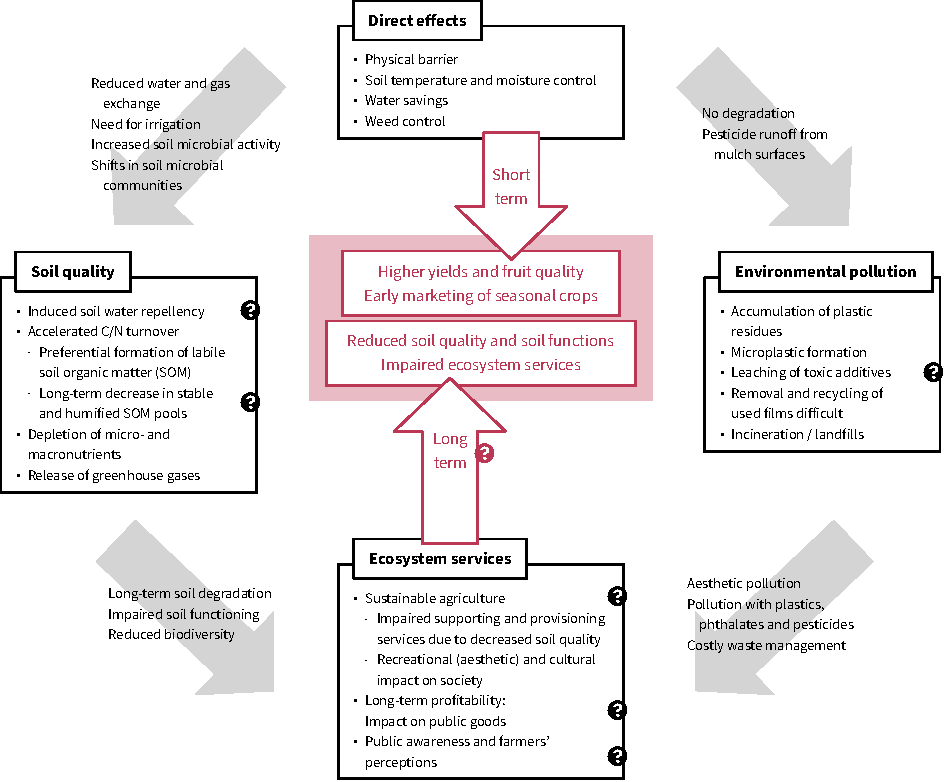
\includegraphics[width=\textwidth]{figures/mulching-overview}
	\caption[Schematic representation of the impacts of plastic mulch use on soil quality, pollution, and implications on agronomy and ecosystem services.]{Schematic representation of the impacts of plastic mulch use on soil quality, pollution, and implications on agronomy and ecosystem services; question marks indicate need for research.}
	\label{fig:mulching-overview}
	\forcerectofloat
\end{figure*}

\section{Conclusions}
\label{sec:plastic-mulching:conclusions}

This literature review identified certain reasons for farmers to apply plastic mulches in agriculture, but it also identified a number of risks and less beneficial effects of plastic mulching with regard to waste treatment, life cycle balance, and impact on soil quality. This includes the persistence of unrecovered plastic mulch in soil, their potential to alter soil quality by shifting the edaphic biocoenosis, accelerating carbon and nitrogen metabolism, as well as potentially degrading \ac{som}. This further includes inducing soil water repellency, increasing the risk of mycotoxin formation in soil and an enhanced release of climate relevant gases. Although several attempts have been made to extend the life cycle of plastic mulches and to reduce their input to soil by recovering and recycling used mulching films, in some cases the cost and effort of these options seem to outweigh their benefits from yield increases, water savings, and facilitated pest control. If, in addition, external effects of mulching on (public) goods or resources like soil quality, biodiversity, or recreation are taken into account, a holistic ecosystem services assessment could make plastic mulching uneconomic and unsustainable.

Comprehensive research with the aim of gaining an extensive understanding of the processes governing the impacts of mulching on soil quality is needed. As most of these biogeochemical processes are not yet sufficiently understood, a final judgment on the implications of plastic mulching for the environment will require long\-/term field experiments combined with targeted process\-/orientated studies on a laboratory scale in order to be able to estimate and potentially avoid environmental risks such as soil degradation. This process understanding is of particular importance for the development of truly biodegradable mulches. In order to assess the contribution of plastic mulching to the pollution with plastic debris and to changes in \ac{som} composition and quality, future research should focus on more detailed soil characterization techniques such as \ac{py-gc-ms} or thermogravimetric approaches as a basis for further impact assessments and life cycle analyses. Similarly, analytical methods which can detect, identify, and quantify plastic debris in soil, need to be developed.

The currently rather unquestioned application of plastic mulching may be attributed to the lack of long\-/term studies and attention in the mass media addressing the potential risks for the soil, biota, and society. Future research should analyze why and under which premises plastic mulching is accepted by farmers, the public, and further stakeholders of the agronomic sector and which long\-/term incentives drive farmers to apply plastic mulches. Deeper knowledge of these aspects would help to make both the agribusiness and society more environment\-/friendly.
